\chapter{Resultat}\label{chap:resultat}

Forrige kapittel presenterte gjennomføring av eksperimentet. Eksperimentet besto av to forsøk hvor en gruppe deltakere gjennomførte forsøket ved hjelp av den digitale prototypen Mine Medisiner og en annen gruppe ved hjelp av pakningsvedlegg. Dette kapittelet presenterer resultatet av eksperimentet og danner grunnlaget for analysen som følger i neste kapittel.

\section{Demografi}

\begin{table}[H]
    \centering
    \begin{tabular}{ | p{3.4cm} | p{3.7cm} | p{3.7cm} |  }
      \hline
        & \textbf{Mine Medisiner} & \textbf{Pakningsvedlegg} \\ \hline
        Alder gj.snitt & 34,5 år & 37,8 år \\ \hline
        Kjønnsfordeling & 4 kvinner - 2 menn  & 4 kvinner - 3 menn \\ \hline
        Ant. legemidler totalt & 10 & 8\\ \hline
        Ant. legemidler gj.snitt &  1,67 & 1,14\\ \hline
        Utdanningsnivå & 2 bachelor (2 IT), 2 master (0 IT), 2 phd (1 IT) & 1 vgs, 4 bachelor (3 IT), 1 master (0 IT), 1 phd (1 IT)\\ \hline
        Datakunnskap gj.snitt & 4,5 av 5 &  4,1 av 5 \\ \hline
    \end{tabular}
    \caption{Demografi}
    \label{tab:demografisammenligning}
\end{table}

Tabell~\ref{tab:demografisammenligning} viser en oversikt over de demografiske fordelingen i forsøksgruppene. Folk i alderen 23 til 70 var representert i begge forsøkene. Aldersgruppen 20-30 år var overrepresentert, noe som førte til lav gjennomsnittsalder for begge forsøkene. 

Det var en liten overvekt av kvinner i begge forsøkene. 

Ingen av deltakerne i eksperimentet brukte mer enn tre legemidler fast, og flere brukte ingen legemidler. Legemiddelforbruket i forsøksgruppen til Mine Medisiner var litt høyere enn i forsøksgruppen til pakningsvedlegg. 

Utdanningsnivået var generelt høyt blant deltakerne, men var i snitt høyere blant deltakergruppen til Mine Medisiner. De fleste deltakerene anså seg selv for å ha god datakunnskap. Dette kan henge sammen med utdanningsnivået blant deltakerne, og at mange av brukerne ble rekruttert fra Institutt for datateknikk og informasjonsvitenskap\footnote{http://www.ntnu.no/web/idi/institutt-for-datateknikk-og-informasjonsvitenskap} ved NTNU. 


\section{Forkunnskap}
\label{sec:forkunnskap}
Deltakerene hadde generelt lav forkunnskap om legemidler. Svært få visste mer om de aktuelle legemidlene enn at Ibux var smertestillende. Betydningen av begrepet \textit{interaksjon} i forbindelse med legemidler var uklart for de fleste deltakerene. 

Det var ingen tydelig sammenheng mellom forkunnskap og hvor riktig deltakerne svarte på utsagnene i forsøket. Det var heller ingen tydelig sammenheng mellom forkunnskap og hvor lang tid deltakerne brukte på å besvare utsagnene.

\section{Vurdering av utsagnene}
Ved hjelp av de respektive systemene tok deltakerene stilling til 7 utsagn. Tabell~\ref{tab:PaastanderPak} og tabell~\ref{tab:PaastanderMed} viser tid og fordeling mellom riktige og gale svar for hvert kasus. De to siste radene i hver tabell viser gjennomsnitt og standardavvik for de ulike variablene. 

\begin{table}[H]
    \centering
    \begin{tabular}{ | p{2cm} | p{2cm} | p{2cm} | p{2cm} | p{2cm} | }
      \hline
       \textbf{Deltaker nr.} & \textbf{Tid (mm:ss)} & \textbf{Prosent riktig} & \textbf{Prosent galt} & \textbf{Prosent "vet ikke"} \\ \hline
        1 & 10:38 & 100\% & 0\% & 0\% \\ \hline
        2 & 10:11 & 57\% & 29\% & 14\% \\ \hline
        4 & 13:30 & 43\% & 14\% & 43\% \\ \hline
        5 & 26:54 & 57\% & 29\% & 14\% \\ \hline
        6 & 11:17 & 86\% & 14\% & 0\% \\ \hline
        12 & 04:33 & 100\% & 0\% & 0\% \\ \hline
        13 & 36:51 & 100\% & 0\% & 0\% \\ \hline \hline
        \textbf{Gj.snitt} & 16:16 & 78\% & 12\% & 10\% \\ \hline
        \textbf{Std.avvik} & 11:22 & 25\% & 13\% & 16\% \\ \hline
    \end{tabular}
    \caption{Vurdering av utsagnene ved hjelp av pakningsvedlegg}
    \label{tab:PaastanderPak}
\end{table}


\begin{table}[H]
    \centering
    \begin{tabular}{ | p{2cm} | p{2cm} | p{2cm} | p{2cm} | p{2cm} | }
      \hline
       \textbf{Deltaker nr.} & \textbf{Tid (mm:ss)} & \textbf{Prosent riktig} & \textbf{Prosent galt} & \textbf{Prosent "vet ikke"} \\ \hline
        3 & 03:29 & 100\% & 0\% & 0\% \\ \hline
        7 & 04:47 & 71\% & 0\% & 29\% \\ \hline
        8 & 05:39 & 100\% & 0\% & 0\% \\ \hline
        9 & 07:26 & 86\% & 14\% & 0\% \\ \hline
        10 & 03:51 & 86\% & 0\% & 14\% \\ \hline
        11 & 08:00 & 86\% & 0\% & 14\% \\ \hline \hline
        \textbf{Gj.snitt} & 05:32 & 88\% & 2\% & 10\% \\ \hline
        \textbf{Std.avvik} & 01:52 & 11\% & 6\% & 12\% \\ \hline
    \end{tabular}
    \caption{Vurdering av utsagnene ved hjelp av Mine Medisiner}
    \label{tab:PaastanderMed}
\end{table}

\section{Læringsutbytte}
Tabell~\ref{tab:LaeringsPak} og tabell~\ref{tab:LaeringsMed} viser resultatet av spørsmålene som undersøkte læringsutbytte. Tabellene viser i hvilken grad deltakerne klarte å gjengi informasjon de brukte til å besvare utsagnene. Den viser også hvor mye deltakerne lærte utover svarene på utsagnene. Resultatene tar høyde for forkunnskapene til deltakerene ved å bare gi poeng for kunnskap som ikke ble nevnt i svarene på spørsmålene om forkunnskap, jf.~\ref{sec:forkunnskap}. Gjengitt kunnskap kan gi opp til 3 poeng og lært kunnskap kan gi opp til 6 poeng.

\begin{table}[H]
    \centering
    \begin{tabular}{ | p{2.6cm} | p{2.6cm} | p{2.6cm} | }
      \hline
       \textbf{Deltaker nr.} & \textbf{Ant. gjengitt} & \textbf{Ant. lært}\\ \hline
        1 & 1/3 & 0/6\\ \hline
        2 & 0/3 & 1/6 \\ \hline
        4 & 0/3 & 1/6 \\ \hline
        5 & 0/3 & 0/6 \\ \hline
        6 & 1/3 & 1/6\\ \hline
        12 & 3/3 & 2/6\\ \hline
        13 & 1/3 & 2/6 \\ \hline
        \textbf{Gj.snitt} & 0,86 & 0,86 \\ \hline
        \textbf{Std.avvik} & 0,69 & 1,07 \\ \hline
    \end{tabular}
    \caption{Læringsutbytte for pakningsvedlegg}
    \label{tab:LaeringsPak}
\end{table}


\begin{table}[H]
    \centering
    \begin{tabular}{ | p{2.6cm} | p{2.6cm} | p{2.6cm} | }
      \hline
       \textbf{Deltaker nr.} & \textbf{Ant. gjengitt}   & \textbf{Ant. lært}\\ \hline
        3 & 2/3 & 0/6\\ \hline
        7 & 1/3  & 1/6\\ \hline
        8 & 3/3 & 0/6\\ \hline
        9 & 1/3  & 0/6\\ \hline
        10 & 1/3  & 1/6 \\ \hline
        11 & 1/3 & 0/6\\ \hline
        \textbf{Gj.snitt} & 0,33 (14\%) & 1,67 (29\%) \\ \hline
        \textbf{Std.avvik} & 0,52 (6\%) & 0,52 (56\%) \\ \hline
    \end{tabular}
    \caption{Læringsutbytte for Mine Medisiner}
    \label{tab:LaeringsMed}
\end{table}

\section{SUS}
Alle deltakerene fylte ut \acrshort{sus}-skjema etter å tatt stilling til utsagnene. Poengsummen er beregnet etter \acrshort{sus}-standard, jf. delkapittel~\ref{subsec:SUS}. \acrshort{sus}-poengsummene til de to systemene er gjengitt i tabell~\ref{tab:SUS}.

\begin{table}[H]	
	\centering
\begin{subtable}[b]{2in}
    \centering
    \begin{tabular}{ | p{2cm} | p{2cm} | }
      \hline
       \textbf{Deltaker nr.} & \textbf{Poengsum} \\ \hline
        1 & 55\\ \hline
        2 & 67,5 \\ \hline
        4 & 50 \\ \hline
        5 & 57,5 \\ \hline
        6 & 37,5 \\ \hline
        12 & 67,5 \\ \hline
        13 & 27,5\\ \hline \hline
        \textbf{Gj.snitt} & 51,79\\ \hline
        \textbf{Std.avvik} & 14,91 \\ \hline
    \end{tabular}
    \caption{Pakningsvedlegg}
    \label{tab:SUSPak}
\end{subtable}
\quad
\begin{subtable}[b]{2in}
    \centering
    \begin{tabular}{ | p{2cm} | p{2cm} | }
      \hline
       \textbf{Deltaker nr.} & \textbf{Poengsum} \\ \hline
        3 & 87,5\\ \hline
        7 & 80\\ \hline
        8 & 95\\ \hline
        9 & 95\\ \hline
        10 & 75\\ \hline
        11 & 80\\ \hline \hline
        \textbf{Gj.snitt} & 85,42\\ \hline
        \textbf{Std.avvik} & 8,43 \\ \hline
    \end{tabular}
    \caption{Mine Medisiner}
    \label{tab:SUSMineMed}
\end{subtable}
 \caption{SUS-poengsum}\label{tab:SUS}
\end{table}

\section{Reaction Card}
Fra en forhåndsdefinert liste med ord valgte deltakerne de 5 ordene de mente best beskrev det systemet de brukte, jf. ~\ref{sec:reactionCards}. Ordskyene i figur~\ref{fig:ordskyP} og figur~\ref{fig:ordskyMM} viser hvilke ord som ble brukt for å beskrive hvert system. Størrelsen på ordene indikerer hvor mange som valgte hvert ord. Ordenes frekvens er gjengitt i tabell~\ref{tab:reactionPak} og tabell~\ref{tab:reactionMed}. 

\begin{figure}[H]
    \centering
    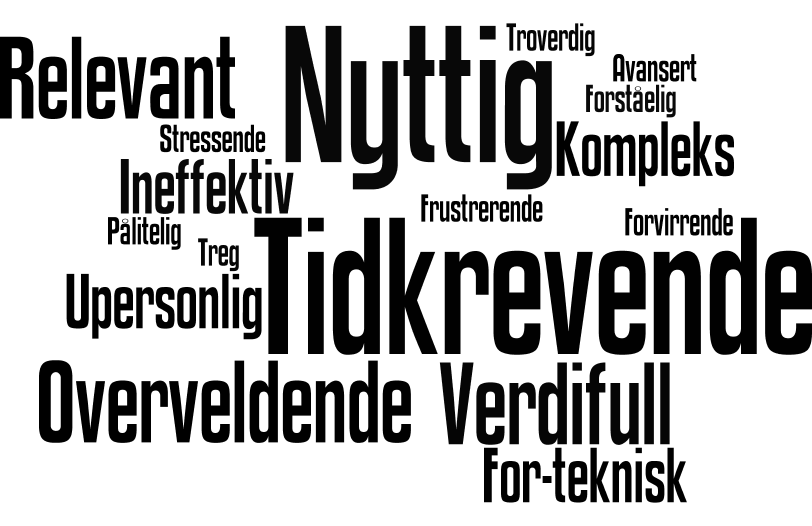
\includegraphics[width=0.8\textwidth]{fig/resultat/ordskyP.png}
    \caption{Ordsky for Reaction Card-oppgave Pakningsvedlegg}
    \label{fig:ordskyP}
\end{figure}

\begin{figure}[H]
    \centering
    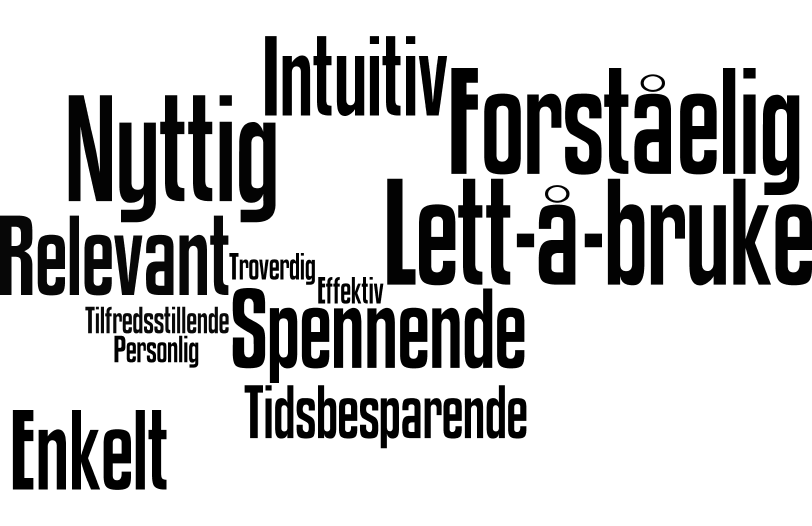
\includegraphics[width=0.8\textwidth]{fig/resultat/ordskyMM.png}
    \caption{Ordsky for Reaction Card-oppgave MineMedisiner}
    \label{fig:ordskyMM}
\end{figure}


\begin{table}
	\centering
	\begin{subtable}[b]{2in}
		\centering
    \begin{tabular}{ | p{2.5cm} | p{1.7cm} | }
      \hline
       \textbf{Ord} & \textbf{Frekvens} \\ \hline
        Nyttig			&		4\\ \hline
        Lett å bruke	&		4\\ \hline
        Intuituv		&	    3\\ \hline
        Enkelt			&		3\\ \hline
        Forståelig		&		4\\ \hline
        Spennende		&		3\\ \hline
        Troverdig		&		1\\ \hline
        Relevant		&		3\\ \hline
        Tilfredsstillende	&	1\\ \hline
        Personlig			&	1\\ \hline
        Tidsbesparende		&	2\\ \hline
        Effektiv			&	1\\ \hline
    \end{tabular}
    \caption{Pakningsvedlegg}
    \label{tab:reactionPak}
	\end{subtable}
	\quad
	\begin{subtable}[b]{2in}
		\centering
    \begin{tabular}{ | p{2.5cm} | p{1.7cm} | }
      \hline
       \textbf{Ord} & \textbf{Frekvens} \\ \hline
        Verdifull			&		3 \\ \hline
        Nyttig				&   	5\\ \hline
        Tidkrevende			&		5\\ \hline
        For teknisk			&		2\\ \hline
        Ineffektiv			&		1\\ \hline
        Relevant			&		3\\ \hline
        Pålitelig			&		1\\ \hline
        Treg				&   	1\\ \hline
        Kompleks			&		2\\ \hline
        Overveldende		&		3\\ \hline
        Troverdig			&		1\\ \hline
        Avansert			&		1\\ \hline
        Upersonlig			&		2\\ \hline
        Ineffektiv			&		1\\ \hline
        Forståelig			&		1\\ \hline
        Frustrerende		&		1\\ \hline
        Forvirrende			&		1\\ \hline
        Stressende			&		1\\ \hline
    \end{tabular}
    \caption{Mine Medisiner}
    \label{tab:reactionMed}
    \end{subtable}
    \caption{Ordfrekvens fra Reaction Cards}\label{table:Ordsky}
\end{table}